\section{Resultados y Análisis}

\begin{frame}
    \frametitle{Comparativas}
    \begin{enumerate}
        \item Se muestran resultados de los experimentos
        \item Hay muchas más comparativas en la sección del apéndice en la memoria principal:
        \begin{itemize}
            \item Figuras de convergencia
            \item Figuras de \textit{boxplots}
            \item Tablas comparativas en todas las métricas (\textit{fitness}, \textit{accuracy}, reducción, tiempo de ejecución, etc.)
            \item Tablas con resultados de los test estadísticos
        \end{itemize}
    \end{enumerate}
\end{frame}

\subsection{Preguntas de Investigación}
\begin{frame}
    \frametitle{Preguntas de Investigación}
    \begin{itemize}
        \item<1-> ¿Merece la pena el uso de algoritmos específicos para la selección de características?
        \item<2-> ¿Cómo se comparan los algoritmos recientes con los clásicos?
        \item<3-> ¿Cuáles de los algoritmos recientes parecen más prometedores?
        \item<4-> ¿Son los algoritmos igualmente eficaces en su versión binaria y continua?
        \item<5-> ¿Cuáles son las opciones más interesantes en ciertos contextos?
    \end{itemize}
\end{frame}

\subsection{Continuos}

\begin{frame}
    \frametitle{Ranking en continuos para fitness: kNN}
    \begin{figure}
        \begin{center}
            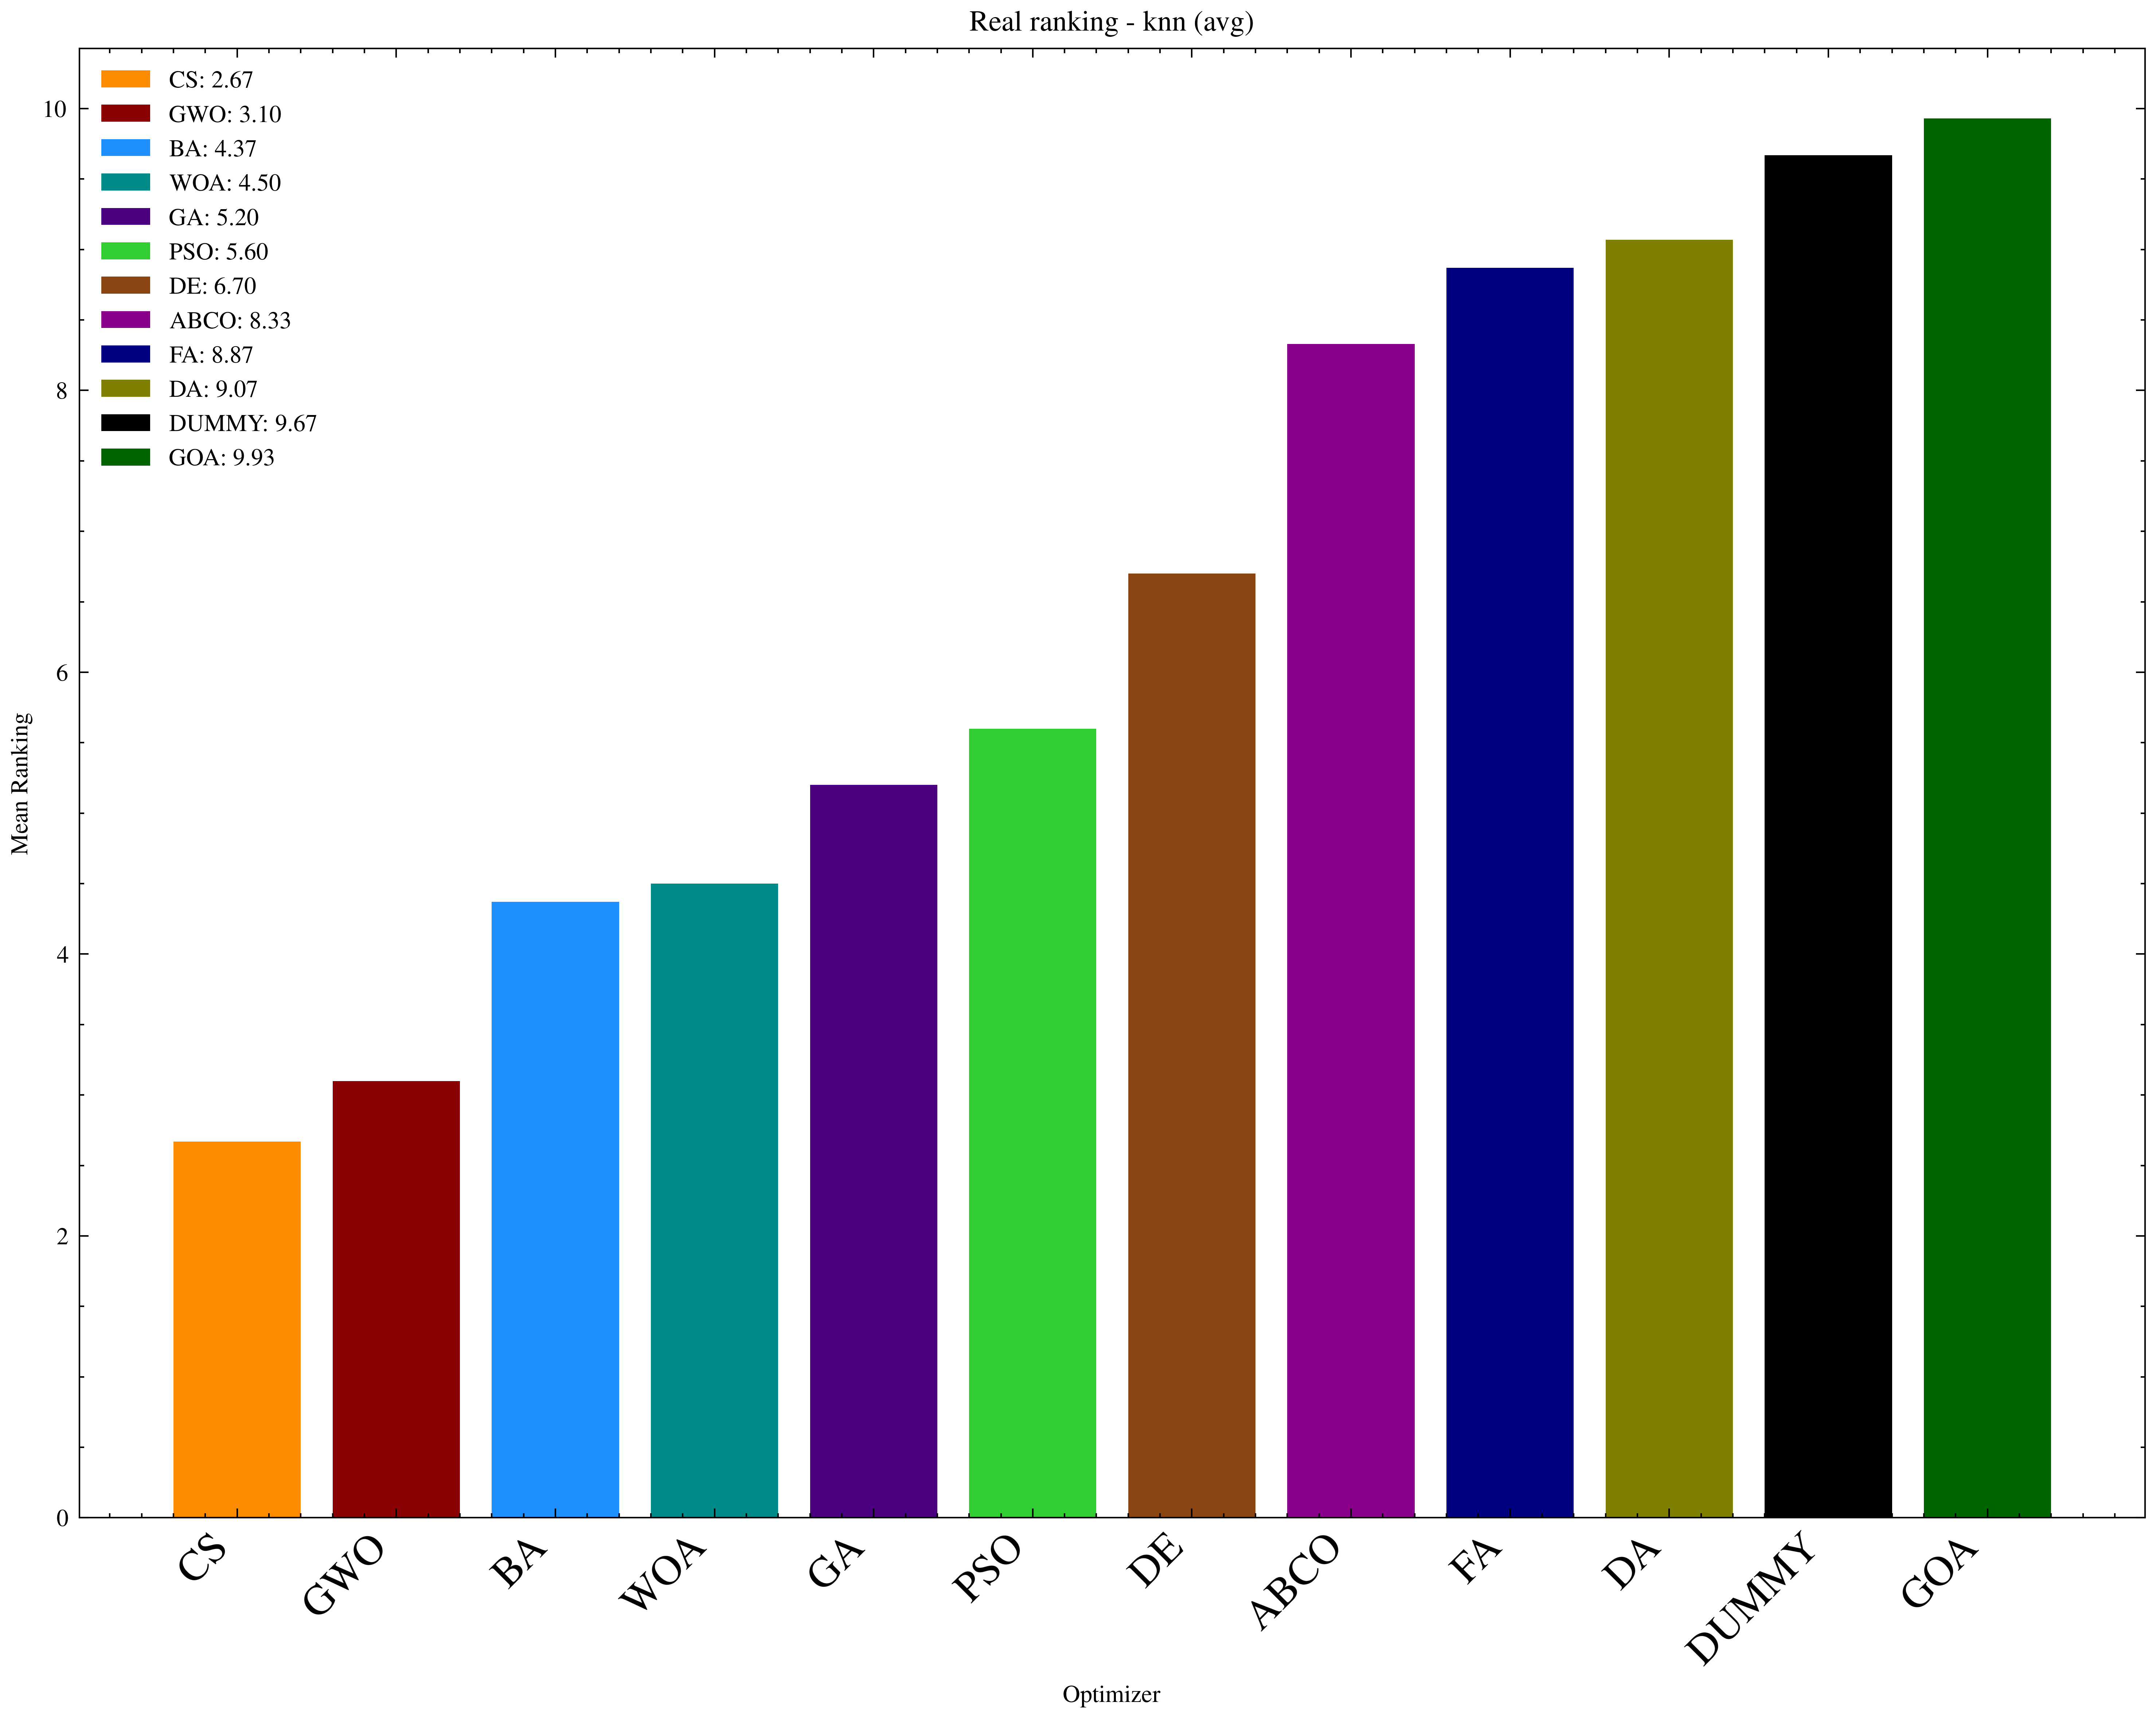
\includegraphics[width=0.45\textwidth]{imagenes/chapter5/rankings_knn_avg_real.png}
        \end{center}
        \caption{Ranking de los algoritmos en versión continua para kNN}
    \end{figure}
\end{frame}
\begin{frame}
    \frametitle{Ranking en continuos para fitness: SVC}
    \begin{figure}
        \begin{center}
            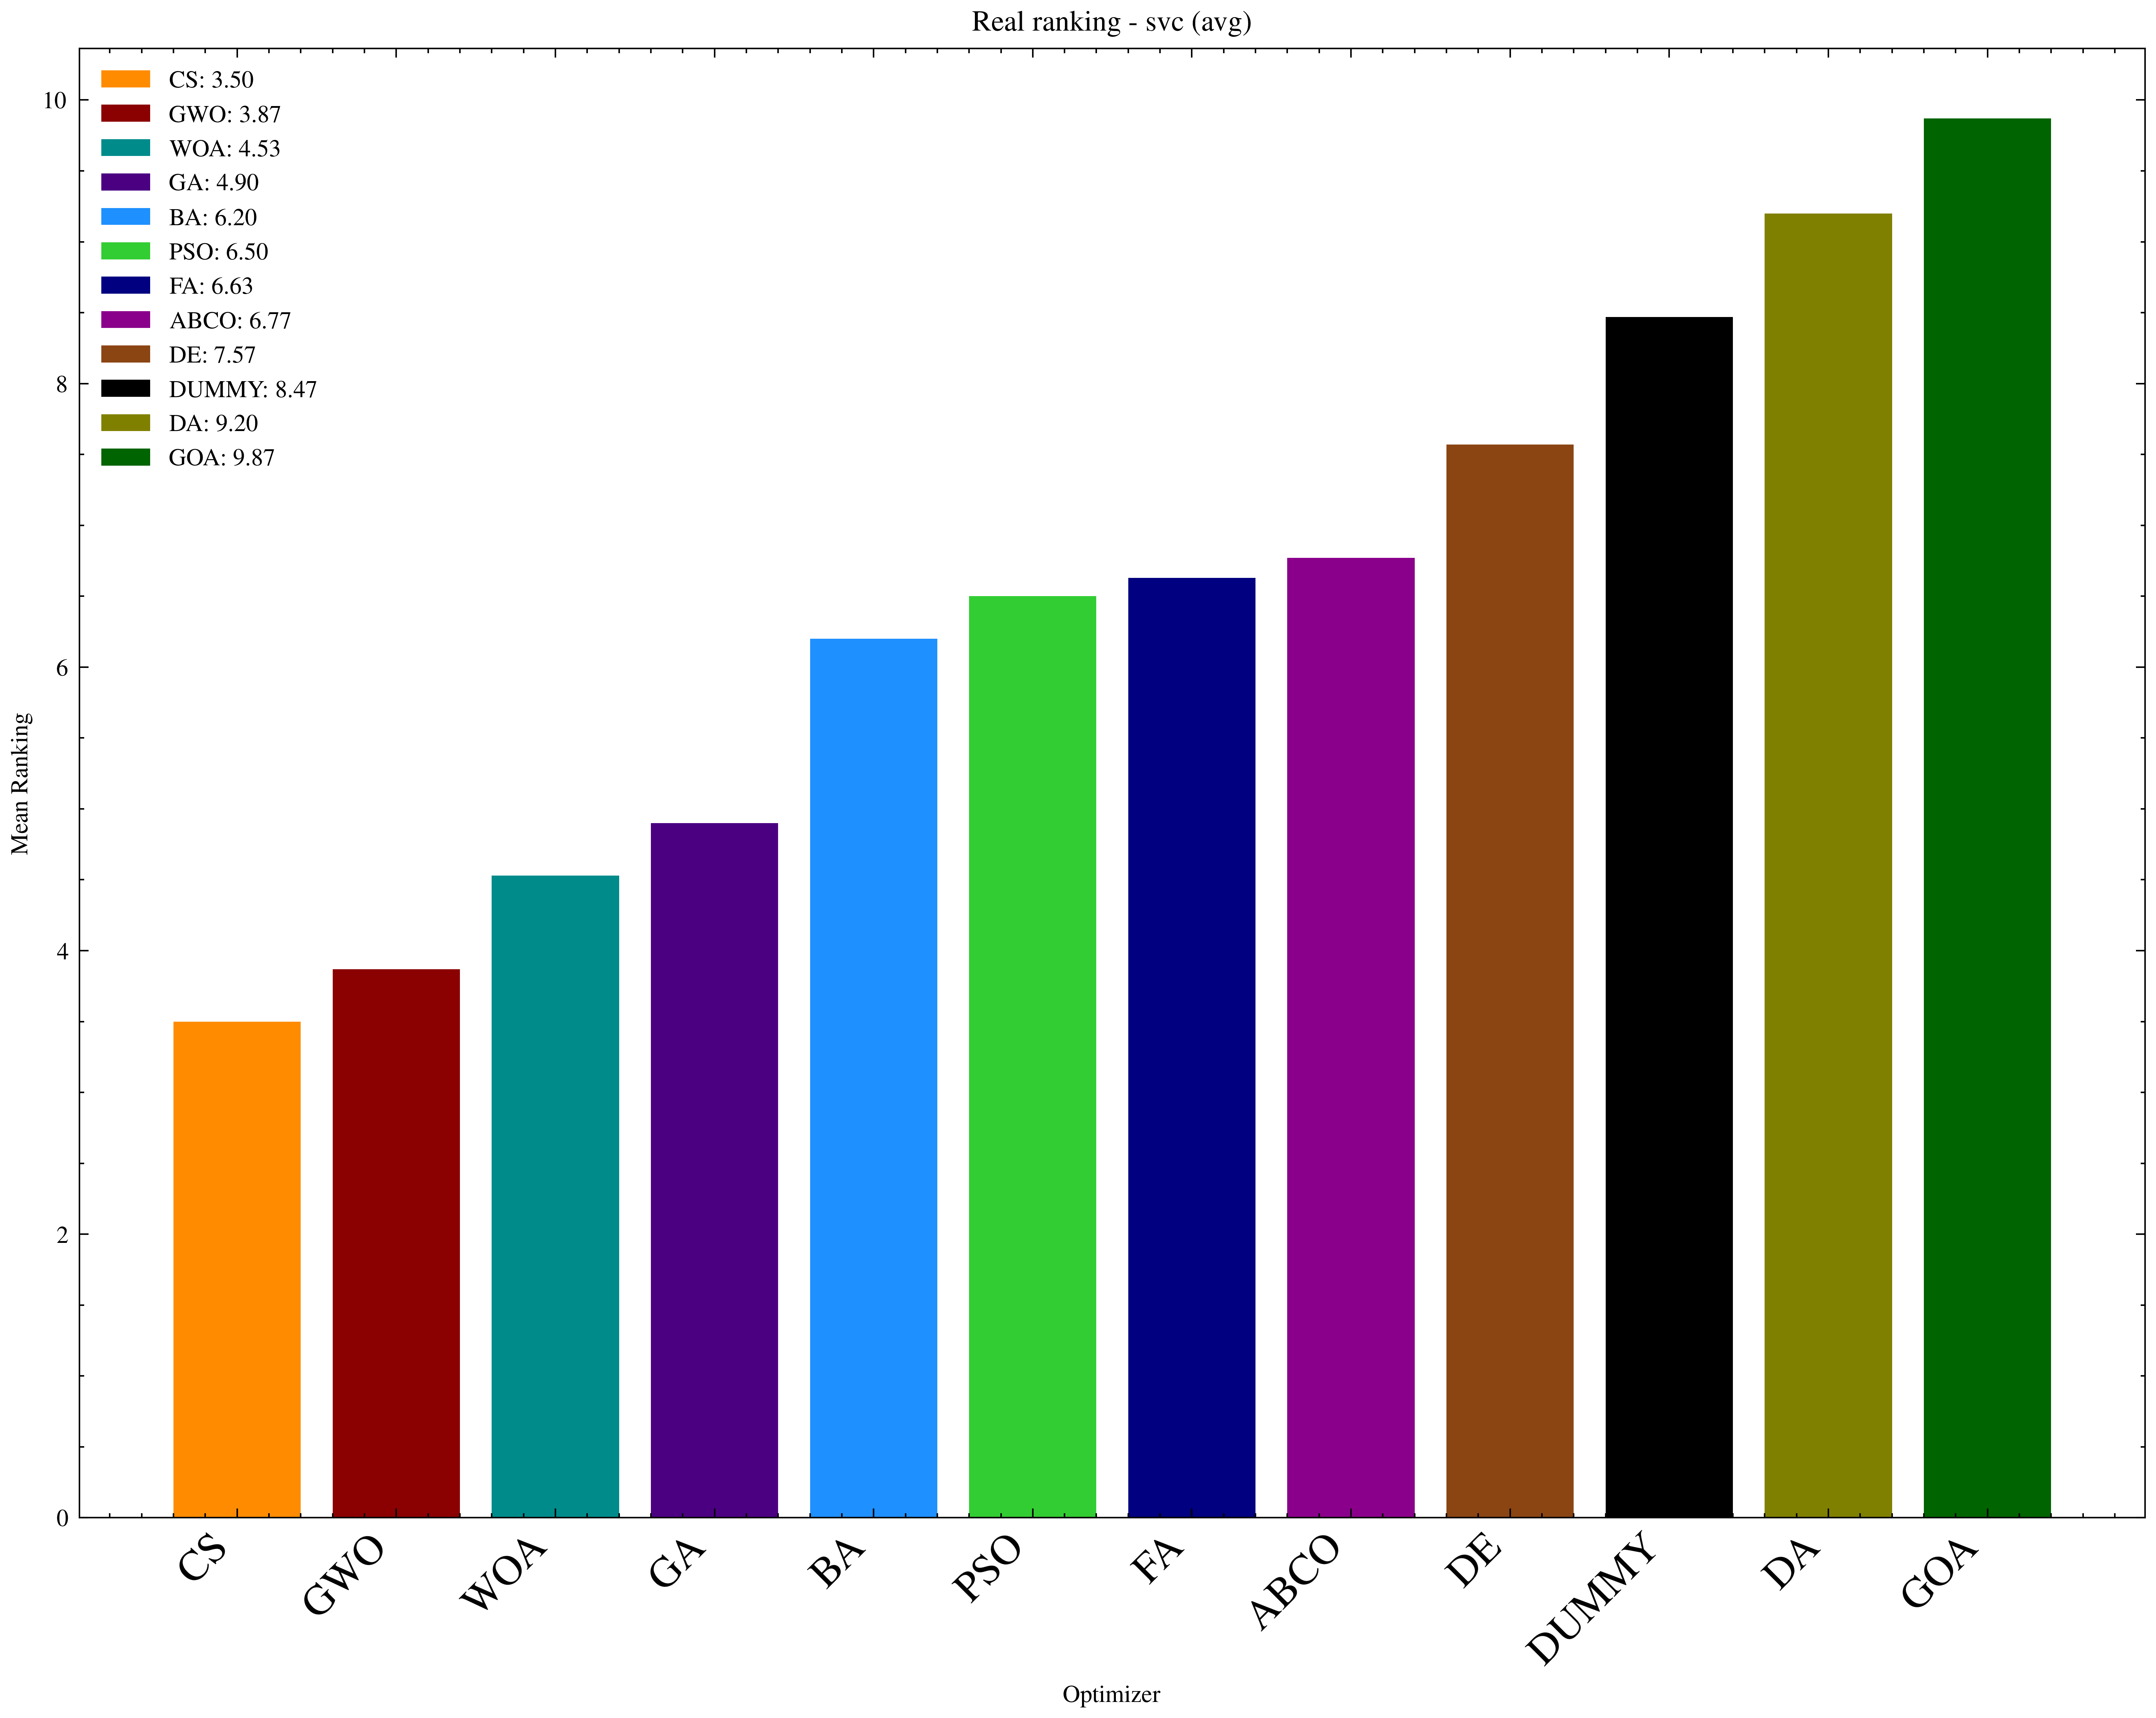
\includegraphics[width=0.45\textwidth]{imagenes/chapter5/rankings_svc_avg_real.png}
        \end{center}
        \caption{Ranking de los algoritmos en versión continua para SVC}
    \end{figure}
\end{frame}

\begin{frame}
    \frametitle{Resultados en continuos}
    \begin{itemize}
        \item<1-> Los mejores algoritmos en \textit{fitness} son:
            \begin{itemize}
                \item<1-> \textcolor{green}{\textbf{CS (Cuckoo Search)}}
                \item<1-> \textcolor{green}{\textbf{GWO (Grey Wolf Optimizer)}}
            \end{itemize}
        \item<2-> Los peores algoritmos son:
            \begin{itemize}
                \item<2-> \textcolor{red}{\textbf{GOA (Grasshopper Optimization Algorithm)}}
                \item<2-> \textcolor{red}{\textbf{DA (Dragonfly Algorithm)}}
            \end{itemize}
        \item<3-> Mejor rendimiento en reducción de características:
            \begin{itemize}
                \item<3-> \textcolor{blue}{\textbf{CS y GWO}} (con mucha diferencia)
            \end{itemize}
        \item<4-> Eficiencia temporal:
            \begin{itemize}
                \item<4-> Más rápido: \textcolor{orange}{\textbf{FA (Firefly Algorithm)}}
                \item<4-> Más lento: \textcolor{purple}{\textbf{ABCO (Artificial Bee Colony Optimization)}}
            \end{itemize}
    \end{itemize}
\end{frame}


\begin{frame}
    \frametitle{Convergencia en continuo: Ionosphere - kNN}
    \begin{figure}[htp]
        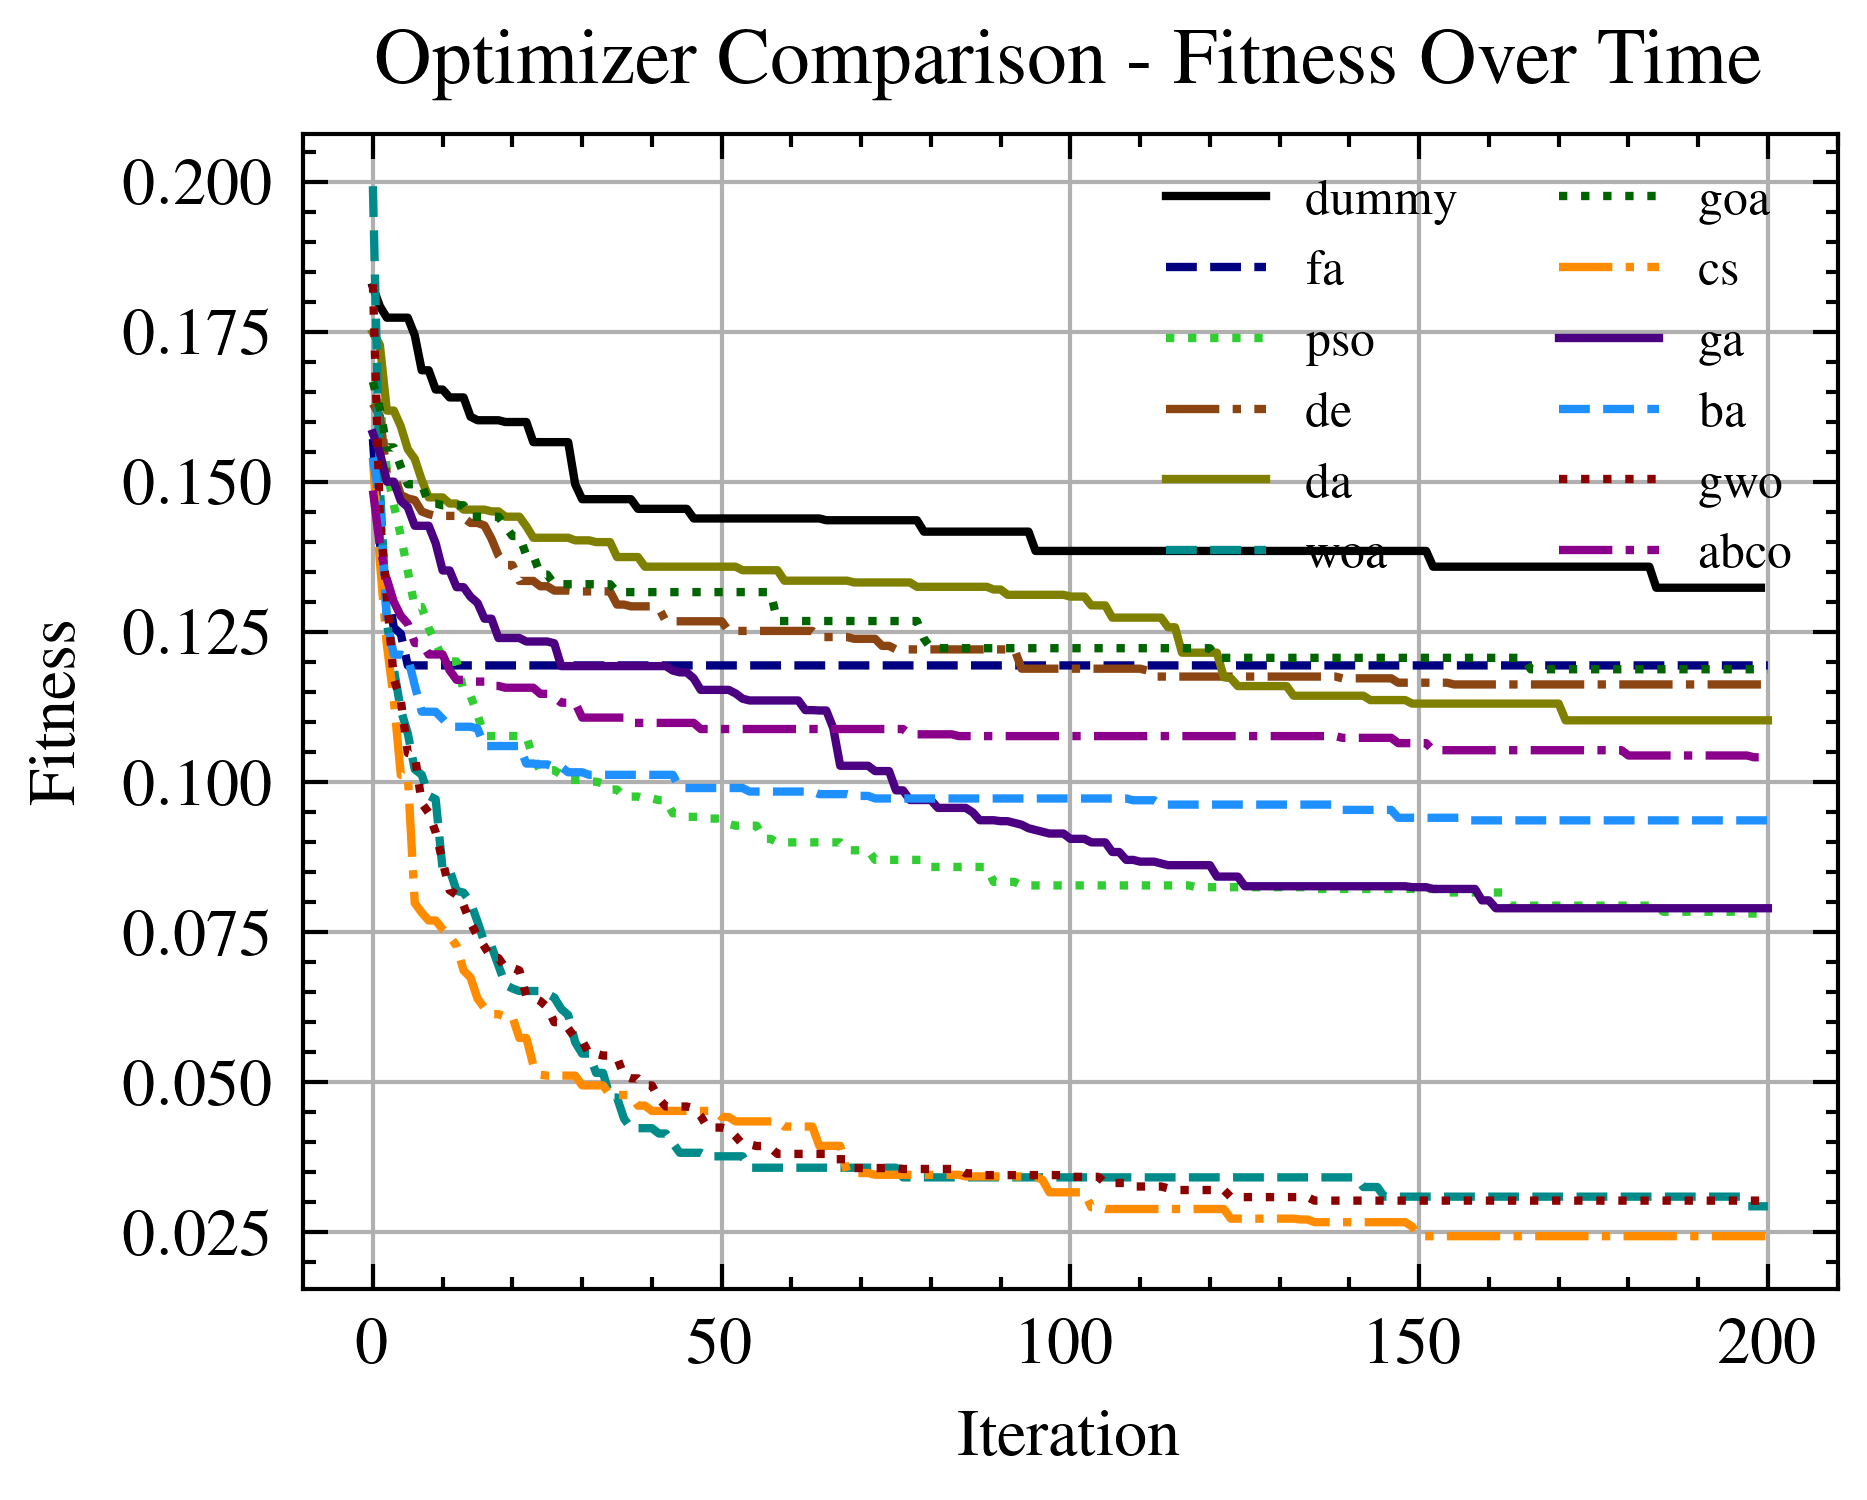
\includegraphics[width=0.45\textwidth]{imagenes/chapter5/optimizers_fitness_knn_io.png}
        \caption{Convergencia de todas las metaheurísticas en ionosphere - knn - real}
    \end{figure}
\end{frame}
\begin{frame}
    \frametitle{Convergencia en continuo: Diabetes - kNN}
    \begin{figure}[htp]
        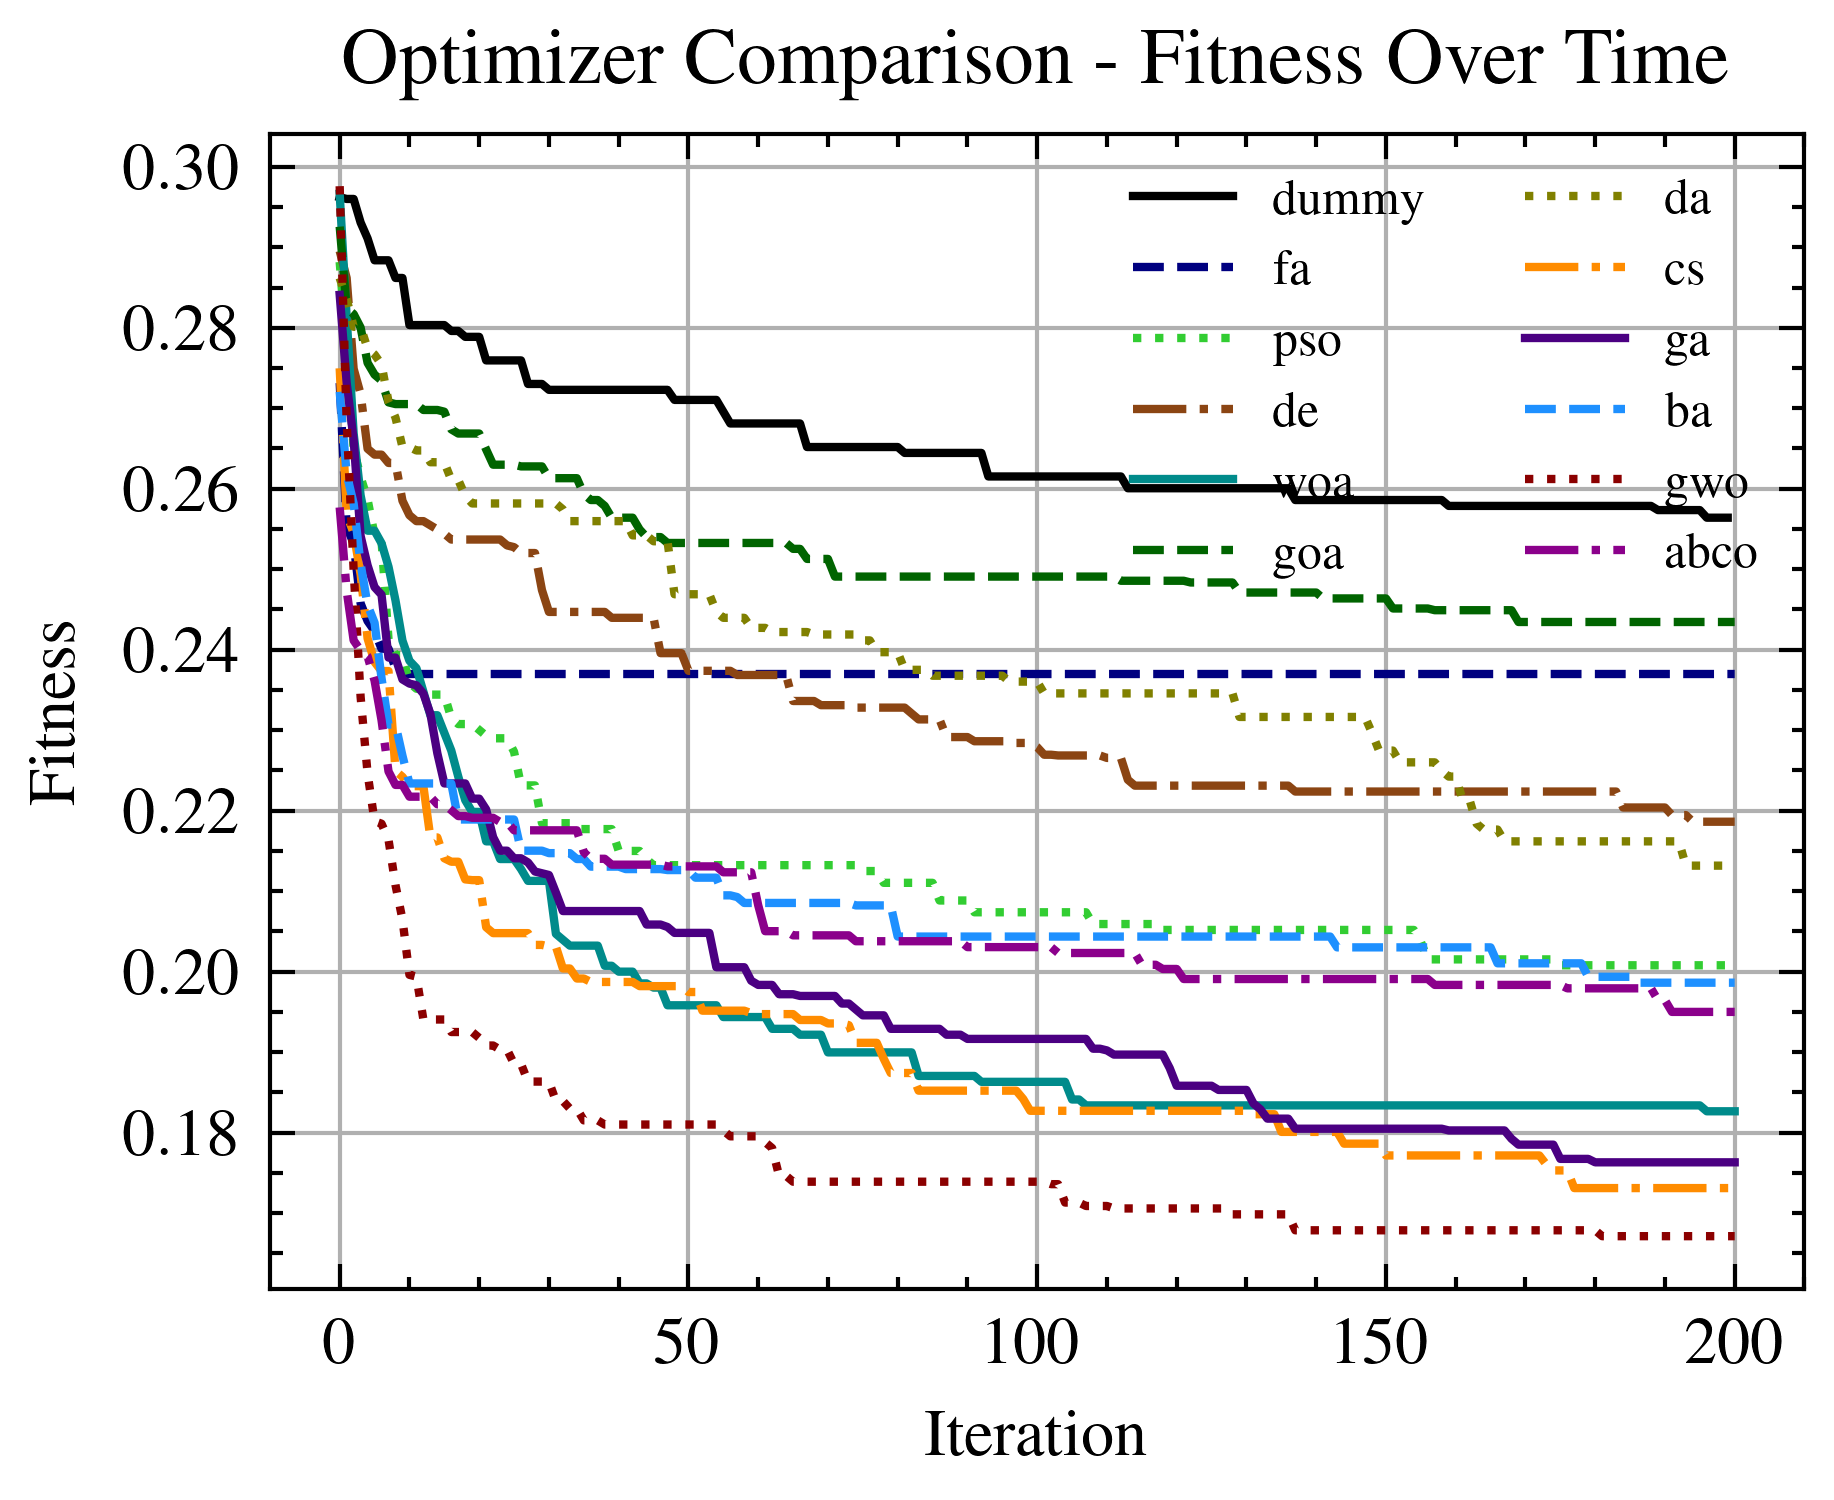
\includegraphics[width=0.45\textwidth]{imagenes/chapter5/optimizers_fitness_knn_dia.png}
        \caption{Convergencia de todas las metaheurísticas en diabetes - knn - real}
    \end{figure}
\end{frame}


\subsection{Binarios}
\begin{frame}
    \frametitle{Ranking en binario para fitness: kNN}
    \begin{figure}
        \begin{center}
            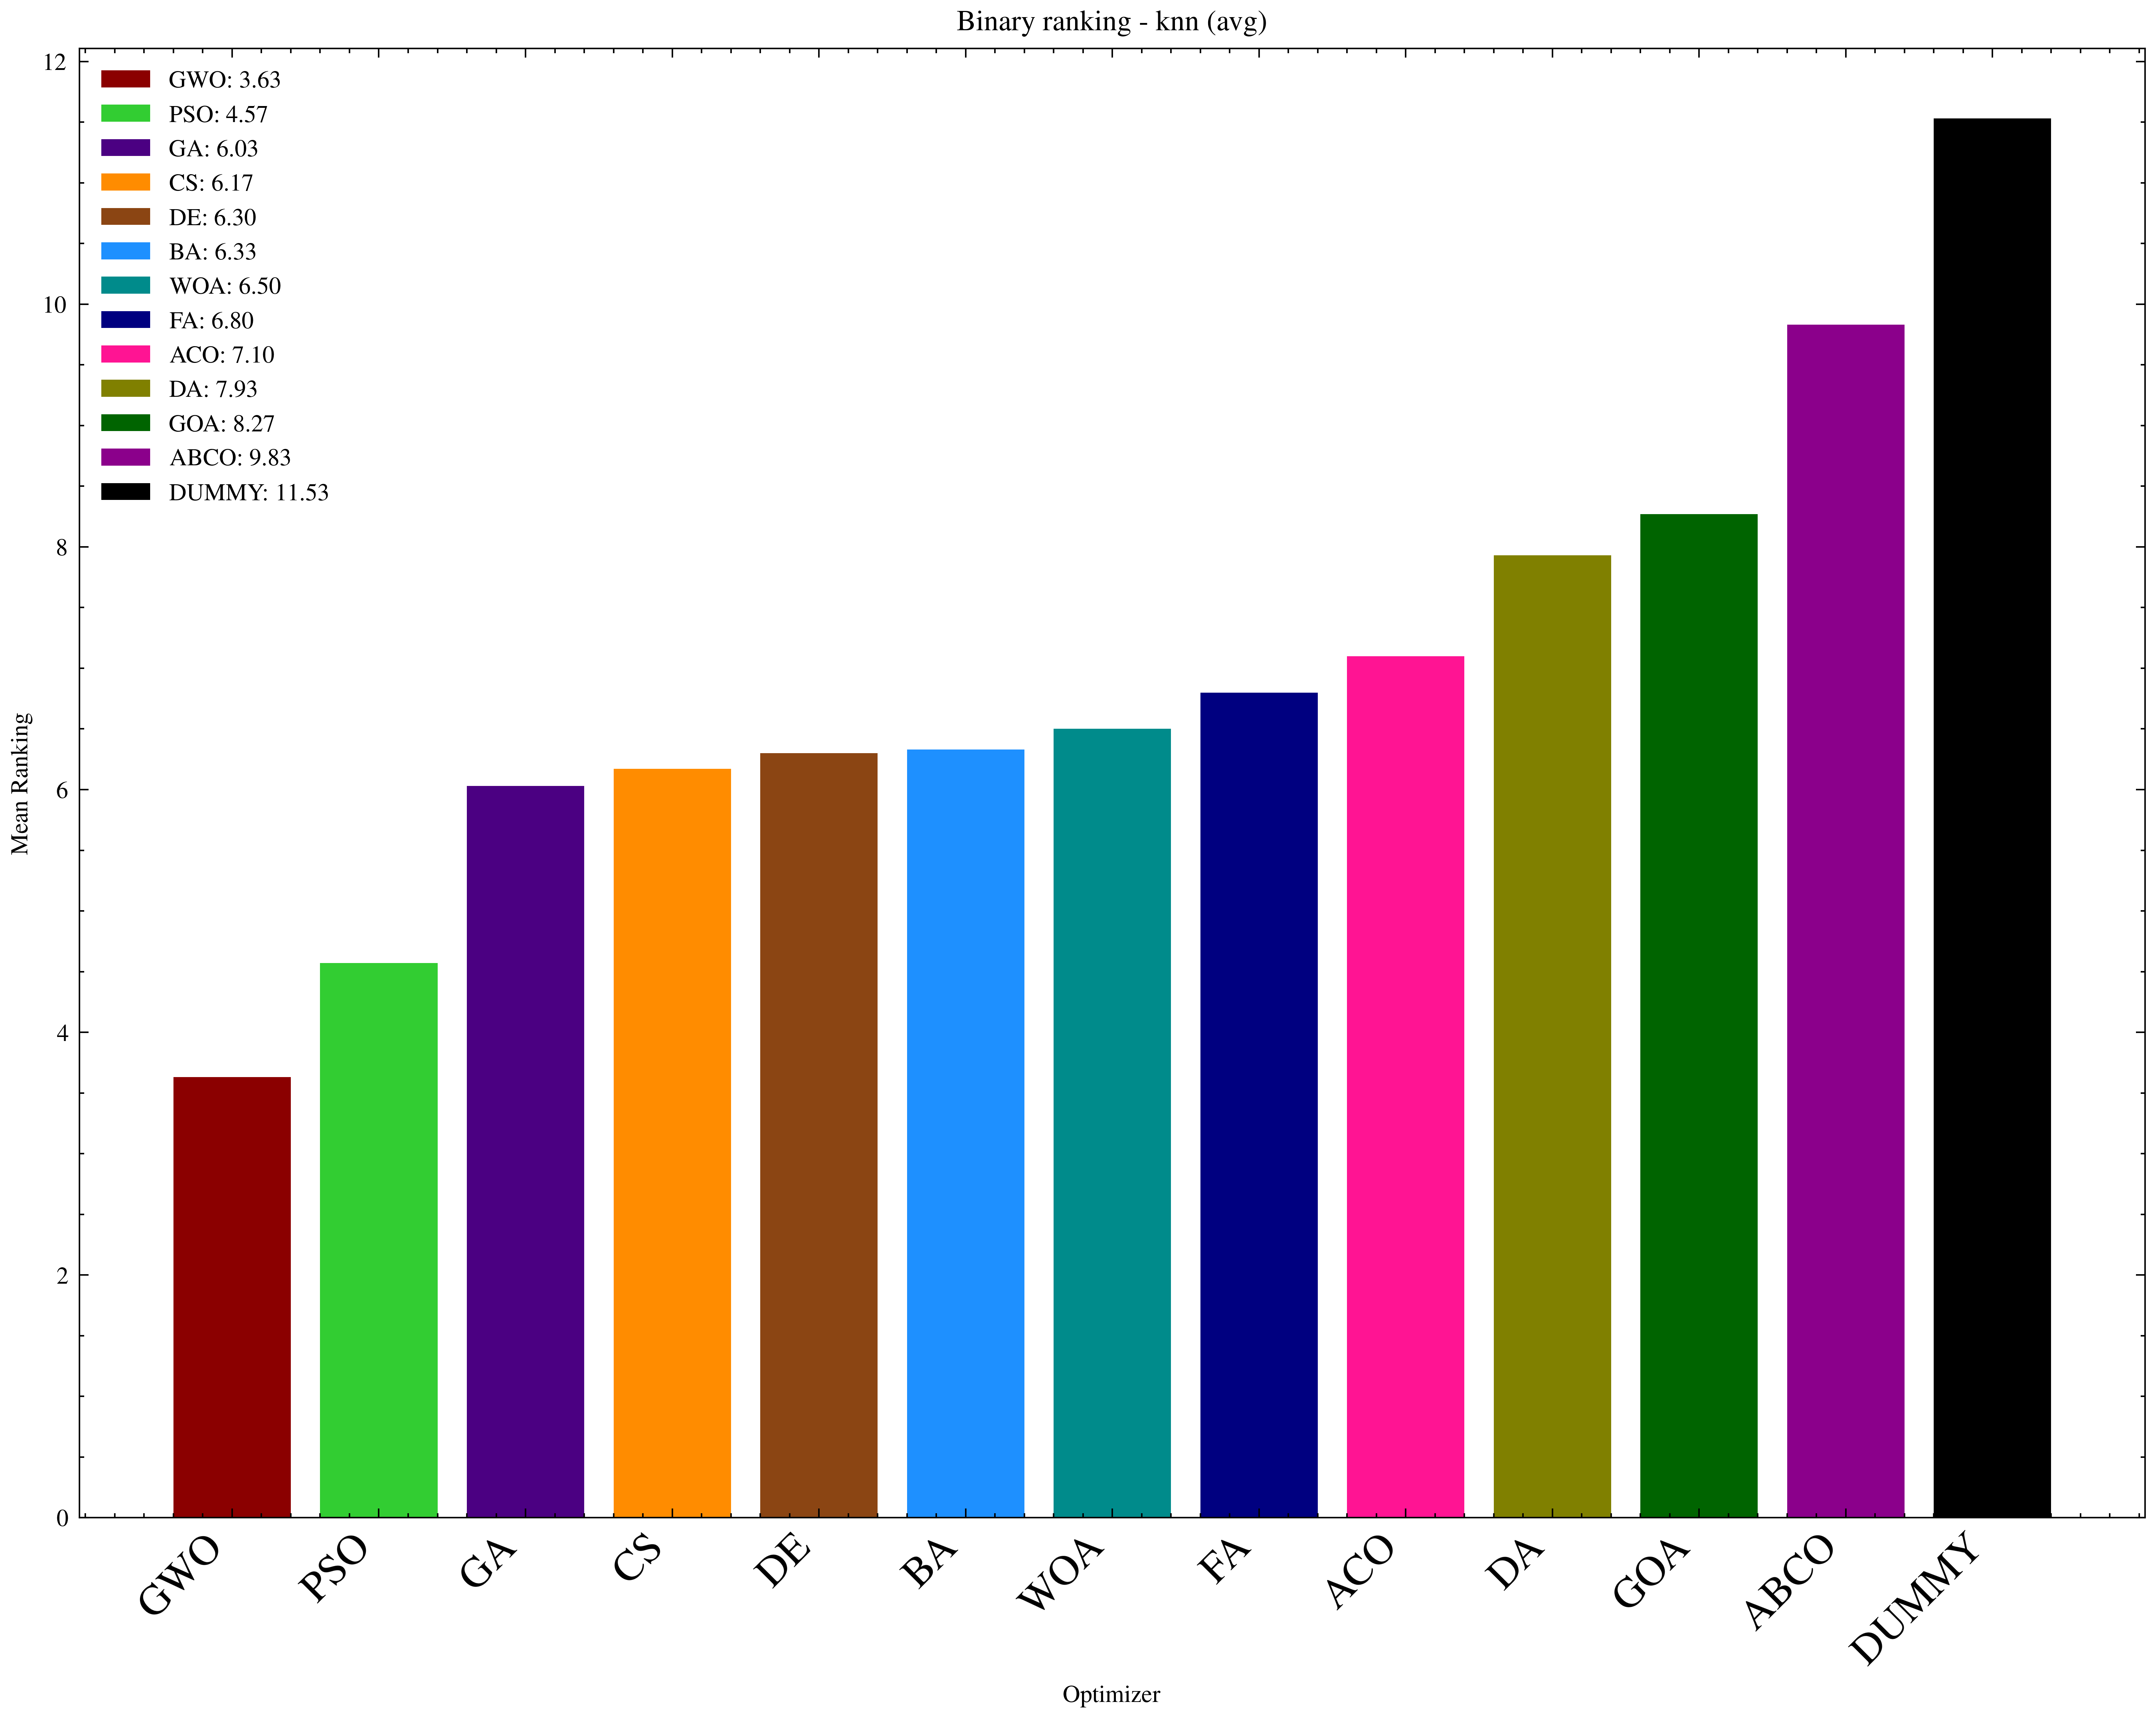
\includegraphics[width=0.45\textwidth]{imagenes/chapter5/rankings_knn_avg_bin.png}
        \end{center}
        \caption{Ranking de los algoritmos en versión binaria para kNN}
    \end{figure}
\end{frame}
\begin{frame}
    \frametitle{Ranking en binario para fitness: SVC}
    \begin{figure}
        \begin{center}
            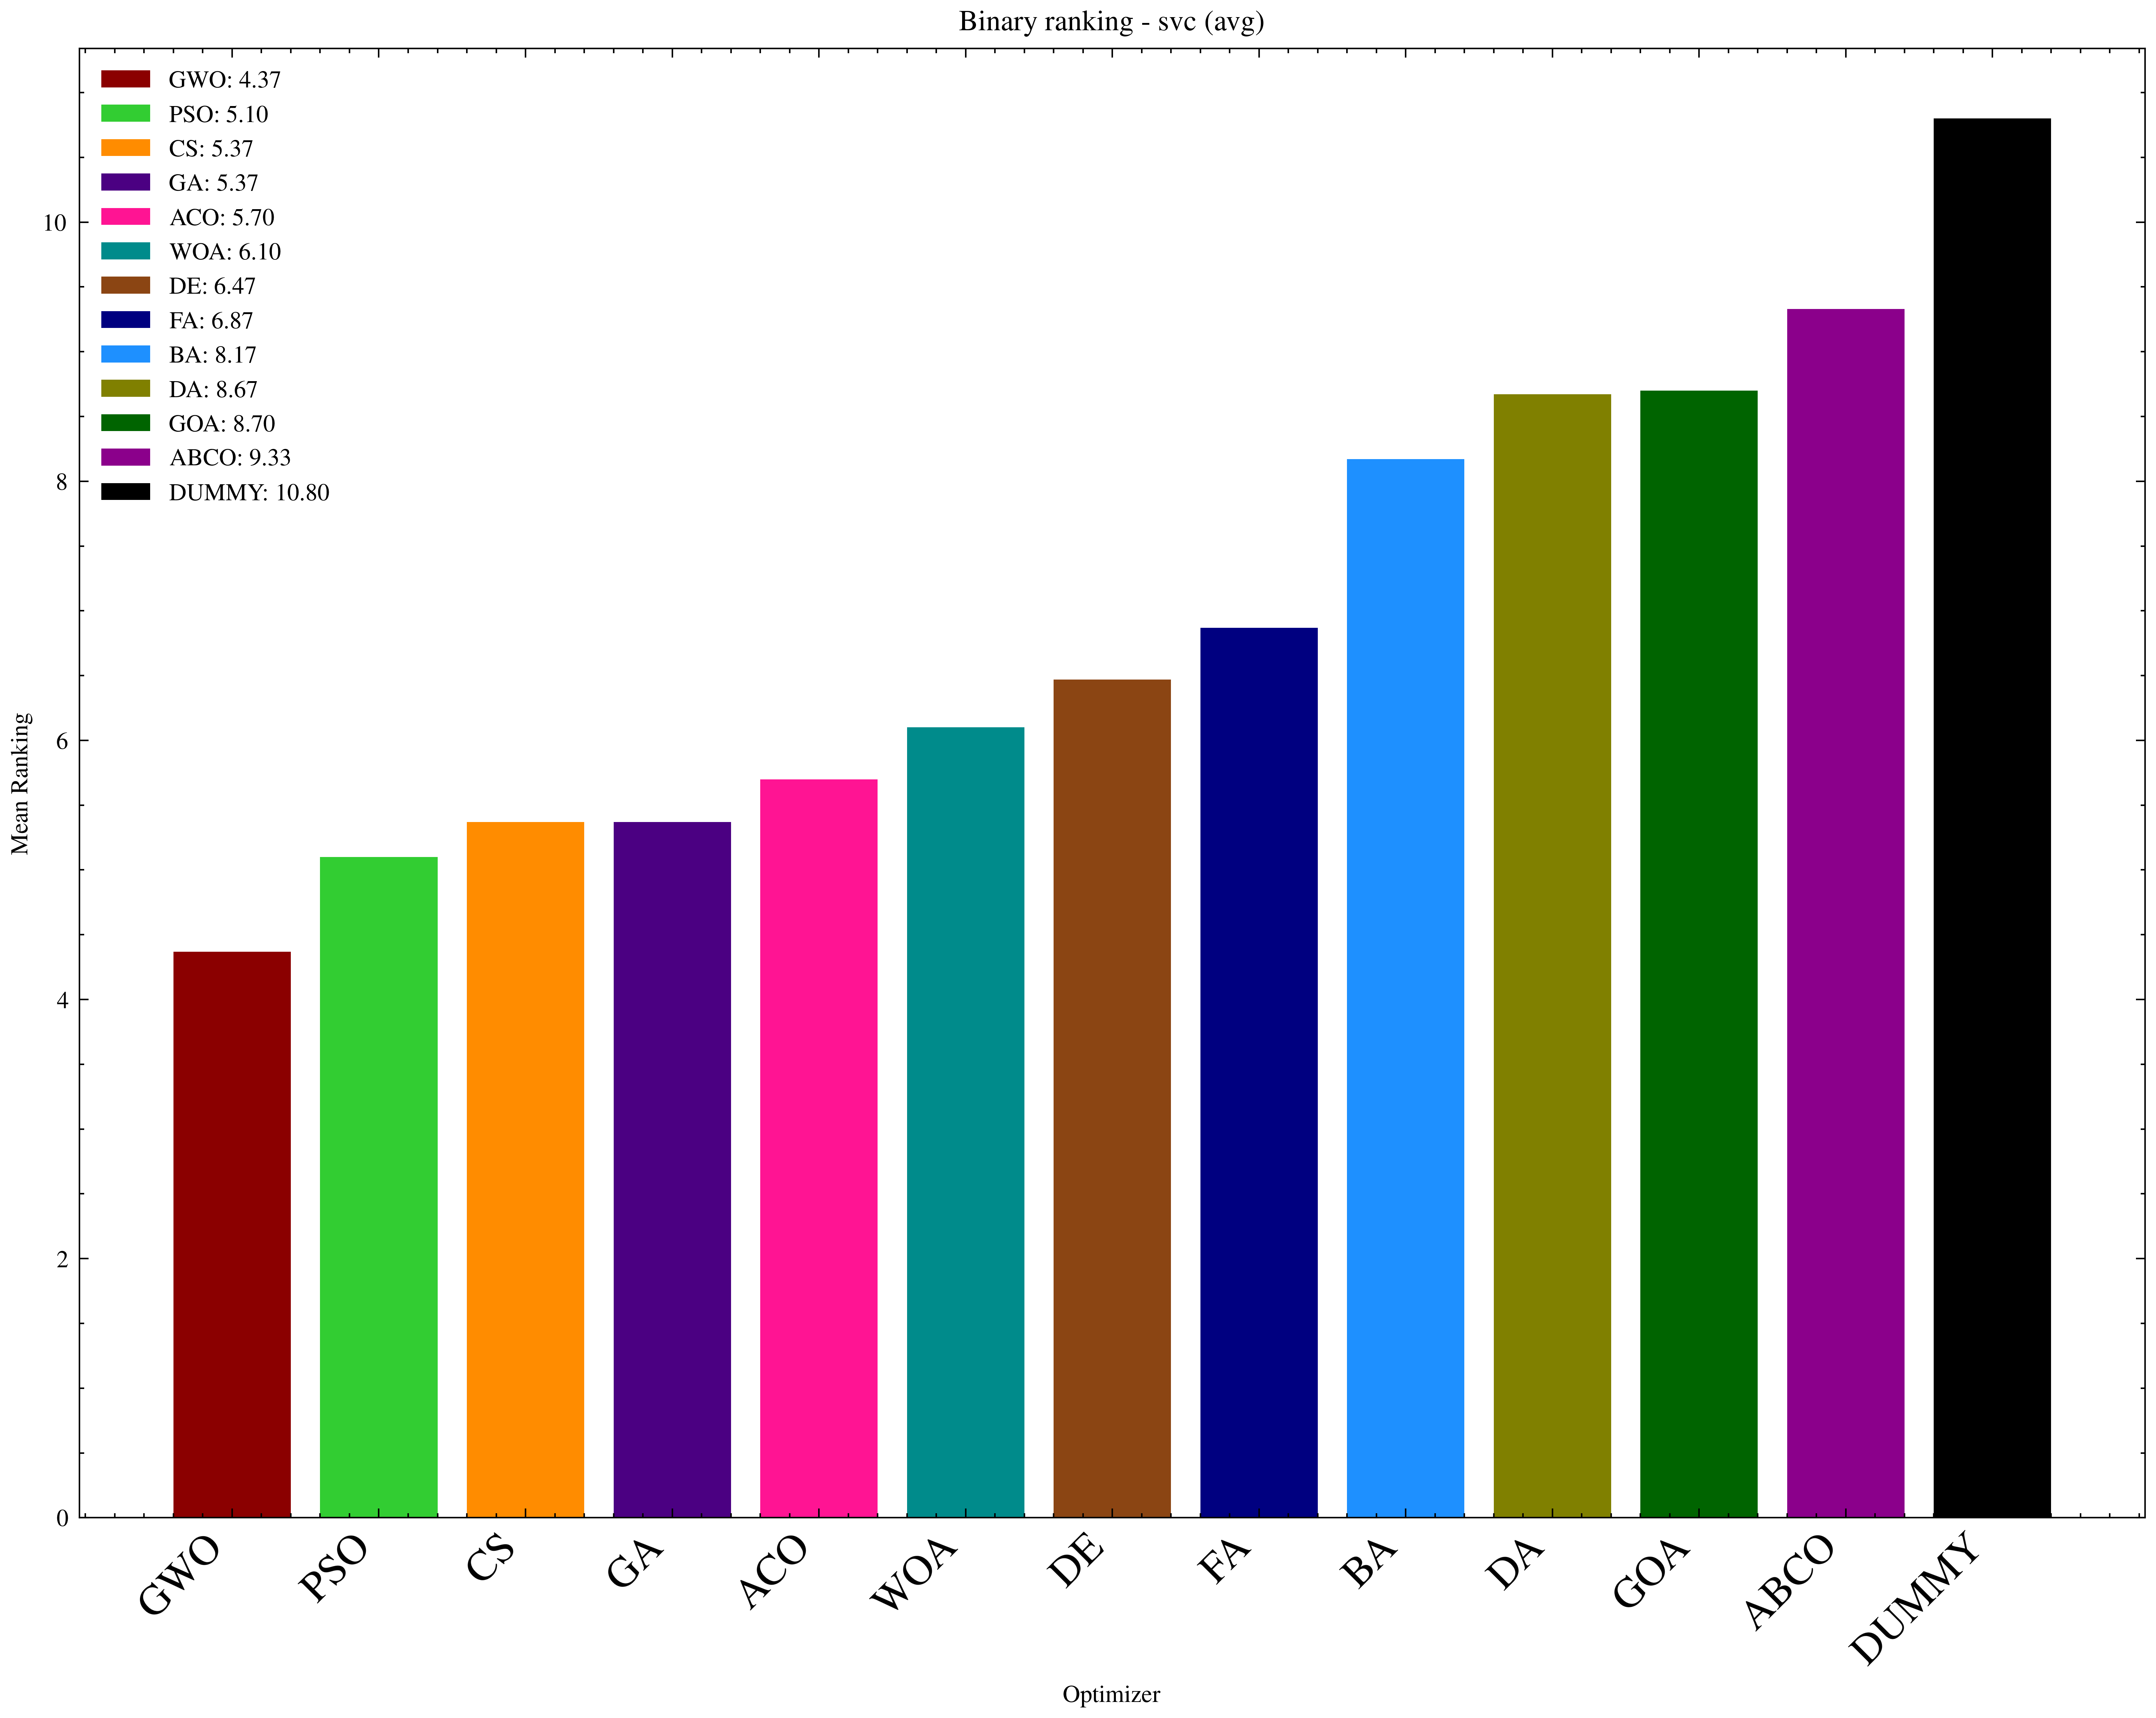
\includegraphics[width=0.45\textwidth]{imagenes/chapter5/rankings_svc_avg_bin.png}
        \end{center}
        \caption{Ranking de los algoritmos en versión binaria para SVC}
    \end{figure}
\end{frame}

\begin{frame}
    \frametitle{Resultados en binarios}
    \begin{itemize}
        \item<1-> Los mejores algoritmos en \textit{fitness} son:
            \begin{itemize}
                \item<1-> \textcolor{green}{\textbf{bGWO (Binary Grey Wolf Optimizer)}}
                \item<1-> \textcolor{green}{\textbf{bPSO (Binary Particle Swarm Optimization)}}
            \end{itemize}
        \item<2-> Los peores algoritmos son:
            \begin{itemize}
                \item<2-> \textcolor{red}{\textbf{bGOA (Binary Grasshopper Optimization Algorithm)}}
                \item<2-> \textcolor{red}{\textbf{bABCO (Binary Artificial Bee Colony Optimization)}}
            \end{itemize}
        \item<3-> Mejor rendimiento en reducción de características:
            \begin{itemize}
                \item<3-> \textcolor{blue}{\textbf{ACO (Ant Colony Optimization)}}
            \end{itemize}
        \item<4-> Eficiencia temporal:
            \begin{itemize}
                \item<4-> Más rápido: \textcolor{orange}{\textbf{bFA (Binary Firefly Algorithm)}}
                \item<4-> Más lento: \textcolor{purple}{\textbf{bABCO (Binary Artificial Bee Colony Optimization)}}
            \end{itemize}
    \end{itemize}
\end{frame}

\subsection{Comparación de resultados}
\begin{frame}
    \frametitle{Comparación de algoritmos específicos vs. originales}
    \begin{columns}
        \column{0.6\textwidth}
        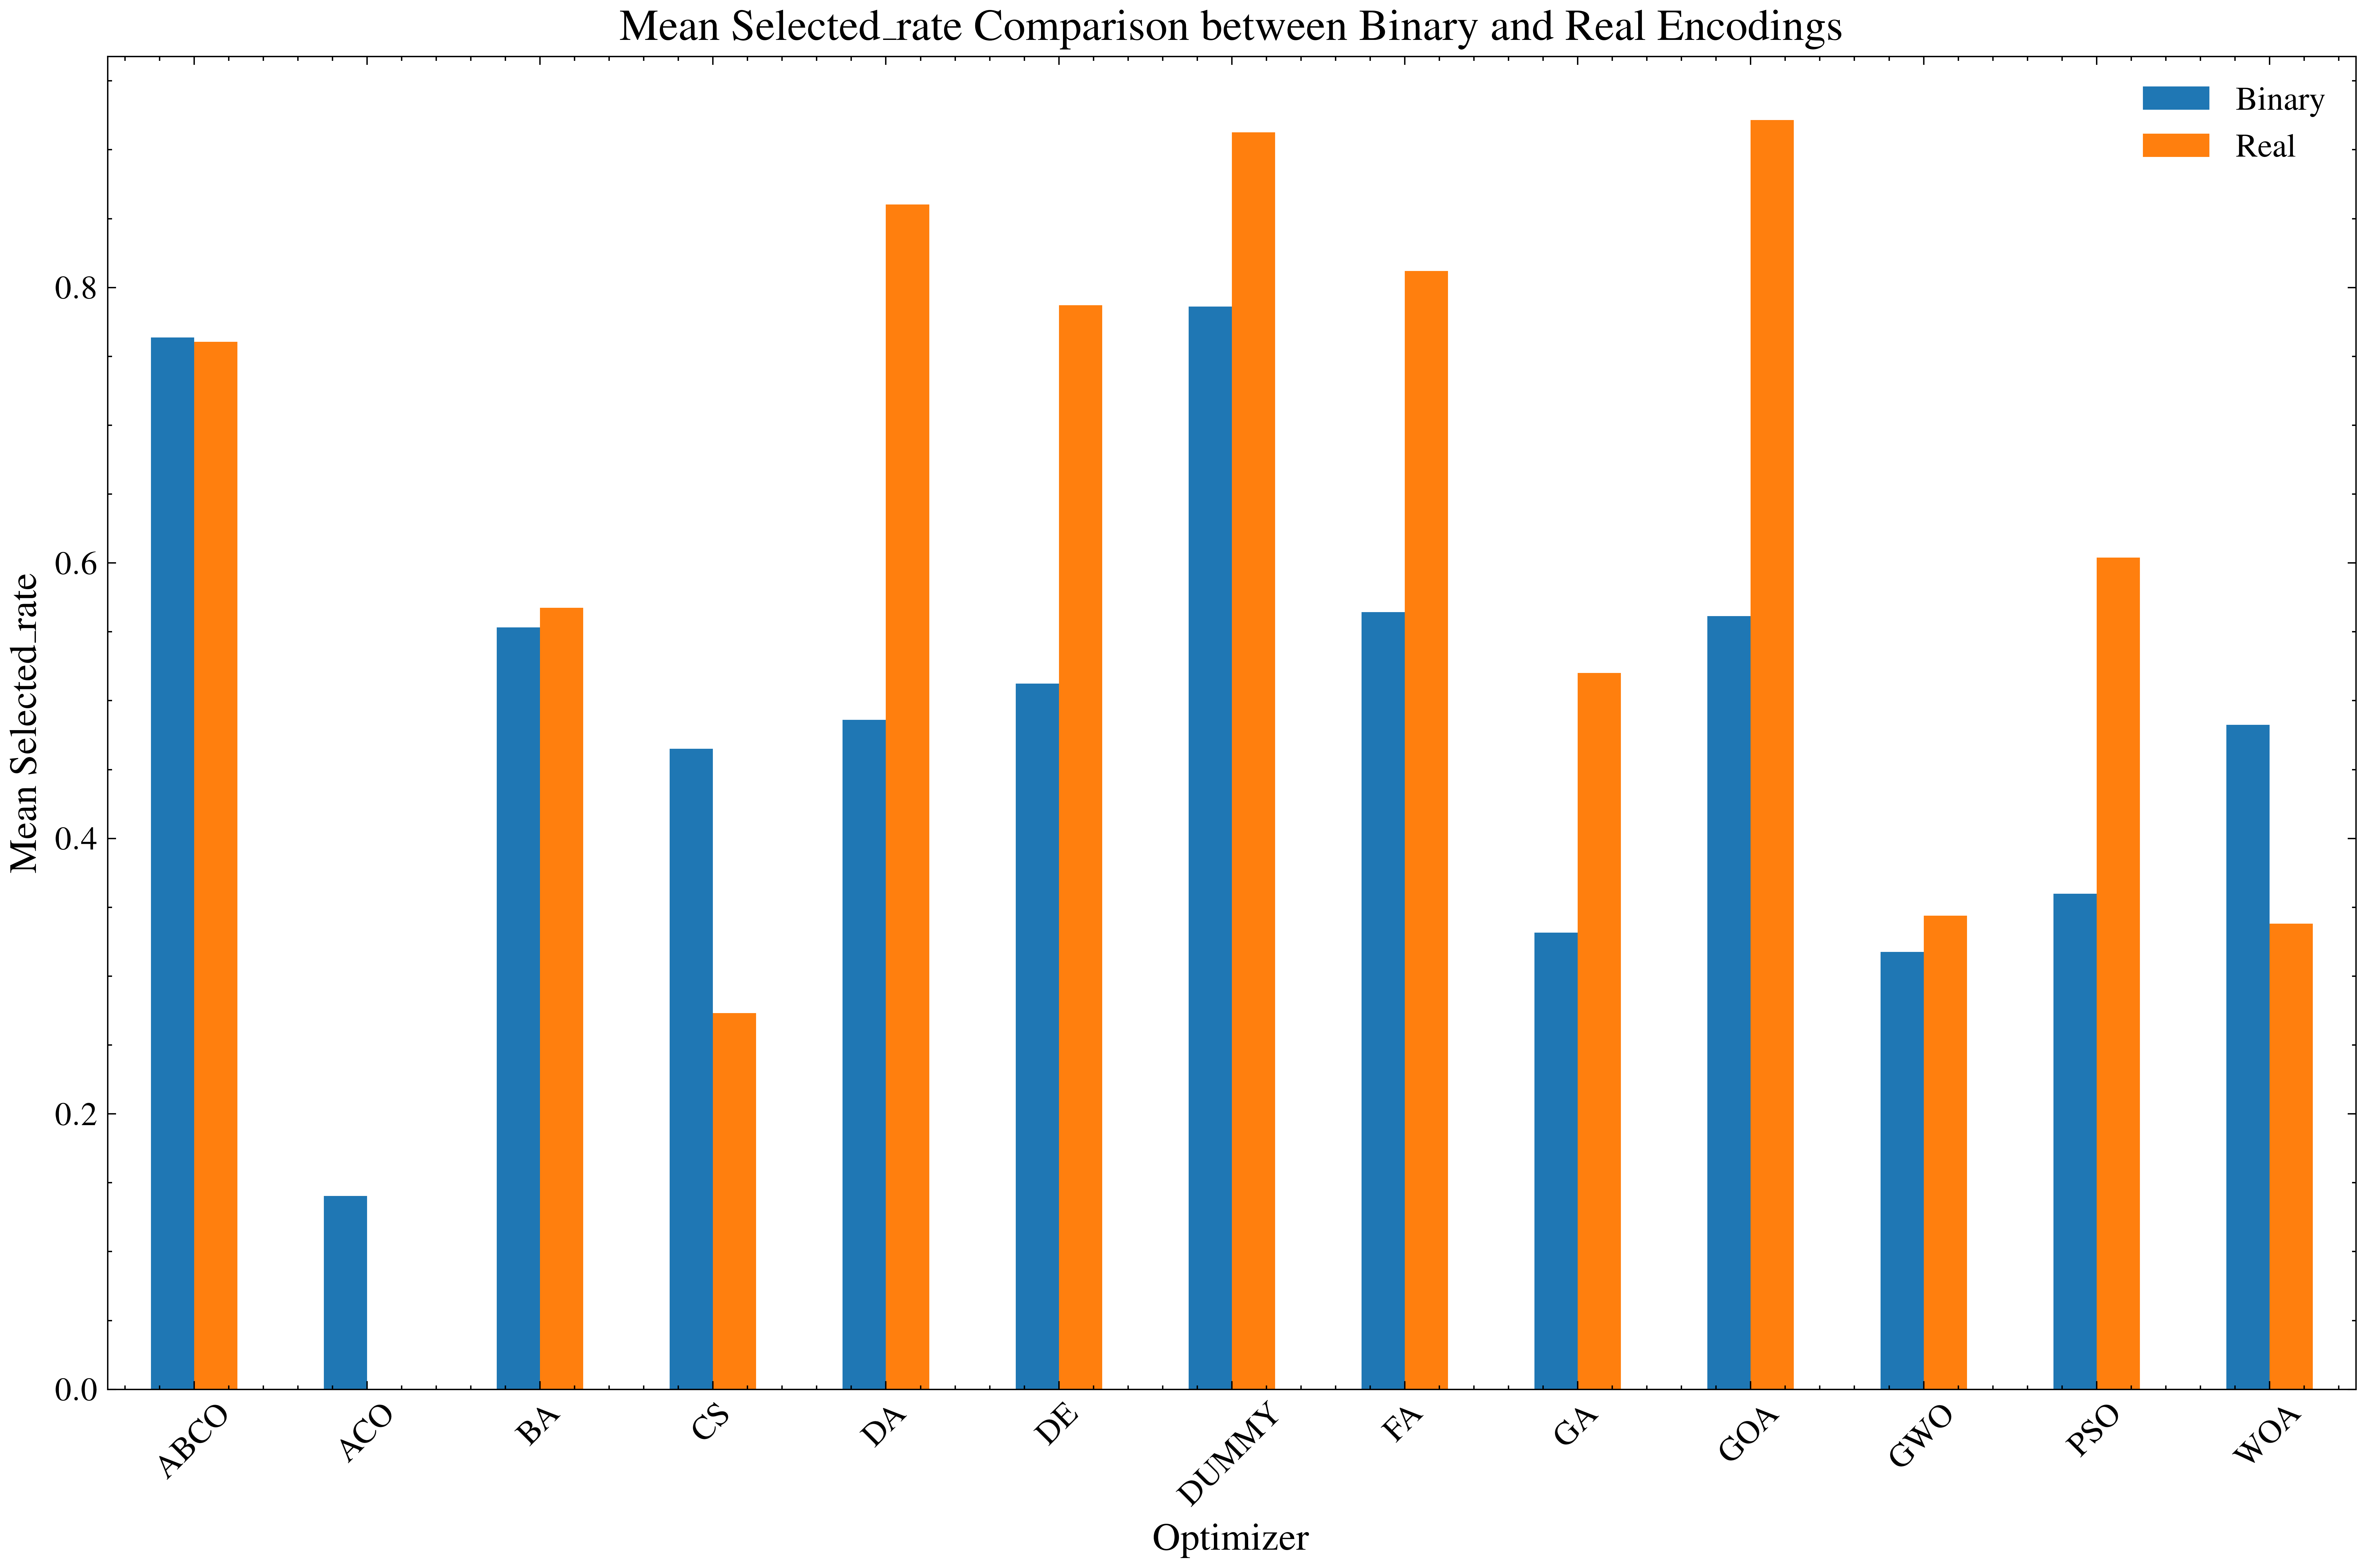
\includegraphics[width=\textwidth]{imagenes/chapter6/selected_rate_comparison.png}
        \column{0.4\textwidth}
        \begin{itemize}
            \item<1-> Los algoritmos binarios tienden a seleccionar menos características
            \item<2-> Algoritmos continuos también capaces de reducir características
            \item<3-> \textcolor{blue}{Conclusión:} Ambos enfoques son válidos para la selección de características, pero los binarios son más eficaces
        \end{itemize}
    \end{columns}
\end{frame}

\begin{frame}
    \frametitle{Comparación de rendimiento: Recientes vs. Clásicos}
    \begin{columns}
        \column{0.6\textwidth}
        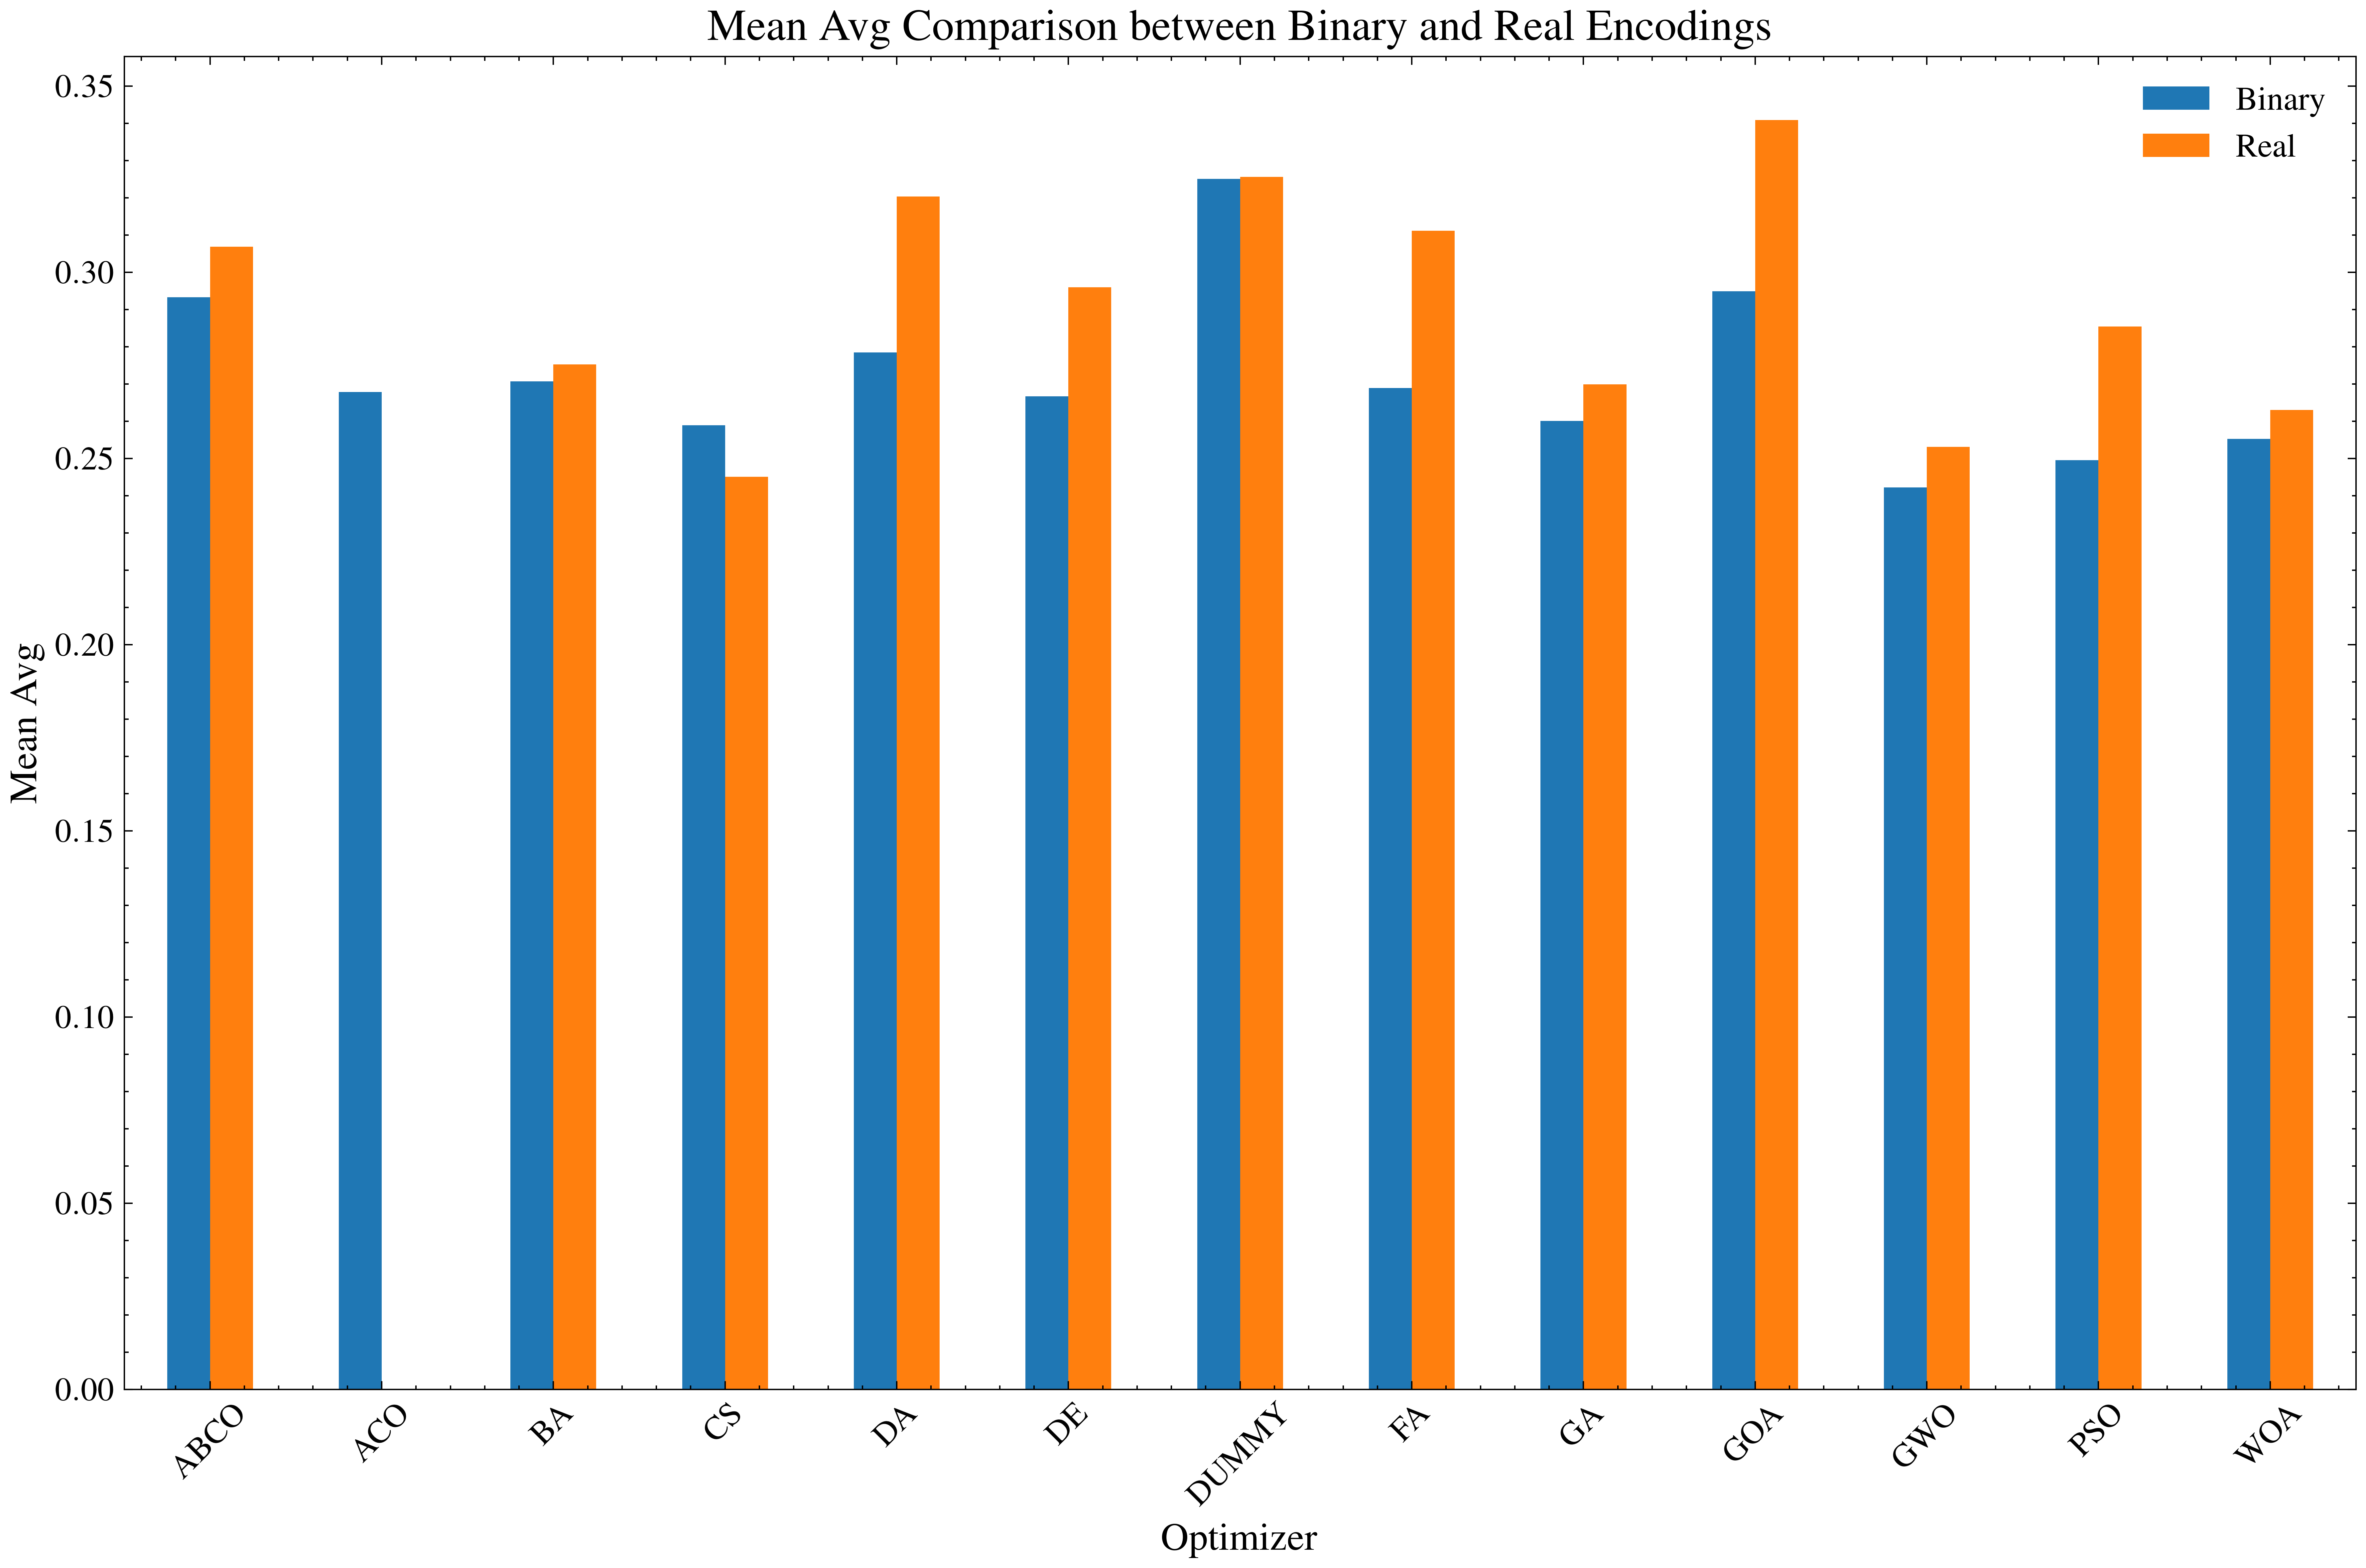
\includegraphics[width=\textwidth]{imagenes/chapter6/avg_comparison.png}
        \column{0.4\textwidth}
        \begin{itemize}
            \item<1-> Algoritmos recientes (GWO, CS) muestran excelente rendimiento
            \item<2-> Algunos clásicos (PSO, DE, GA) siguen siendo competitivos
            \item<3-> \textcolor{blue}{Conclusión:} Algunos recientes ofrecen mejoras, pero los clásicos siguen siendo muy robustos
        \end{itemize}
    \end{columns}
\end{frame}

\begin{frame}
    \frametitle{Algoritmos recientes prometedores}
    \begin{itemize}
        \item<1-> En versiones continuas:
            \begin{itemize}
                \item \textcolor{green}{\textbf{GWO (Grey Wolf Optimizer)}}
                \item \textcolor{green}{\textbf{CS (Cuckoo Search)}}
            \end{itemize}
        \item<2-> En versiones binarias:
            \begin{itemize}
                \item \textcolor{blue}{\textbf{bGWO (Binary Grey Wolf Optimizer)}}
                \item \textcolor{blue}{\textbf{bPSO (Binary Particle Swarm Optimization)}}
            \end{itemize}
        \item<3-> \textcolor{orange}{Conclusión:} GWO destaca en ambas versiones, mostrando gran adaptabilidad y rendimiento
    \end{itemize}
\end{frame}

\begin{frame}
    \frametitle{Eficacia en versiones originales vs. binarias}
    \begin{columns}
        \column{0.6\textwidth}
        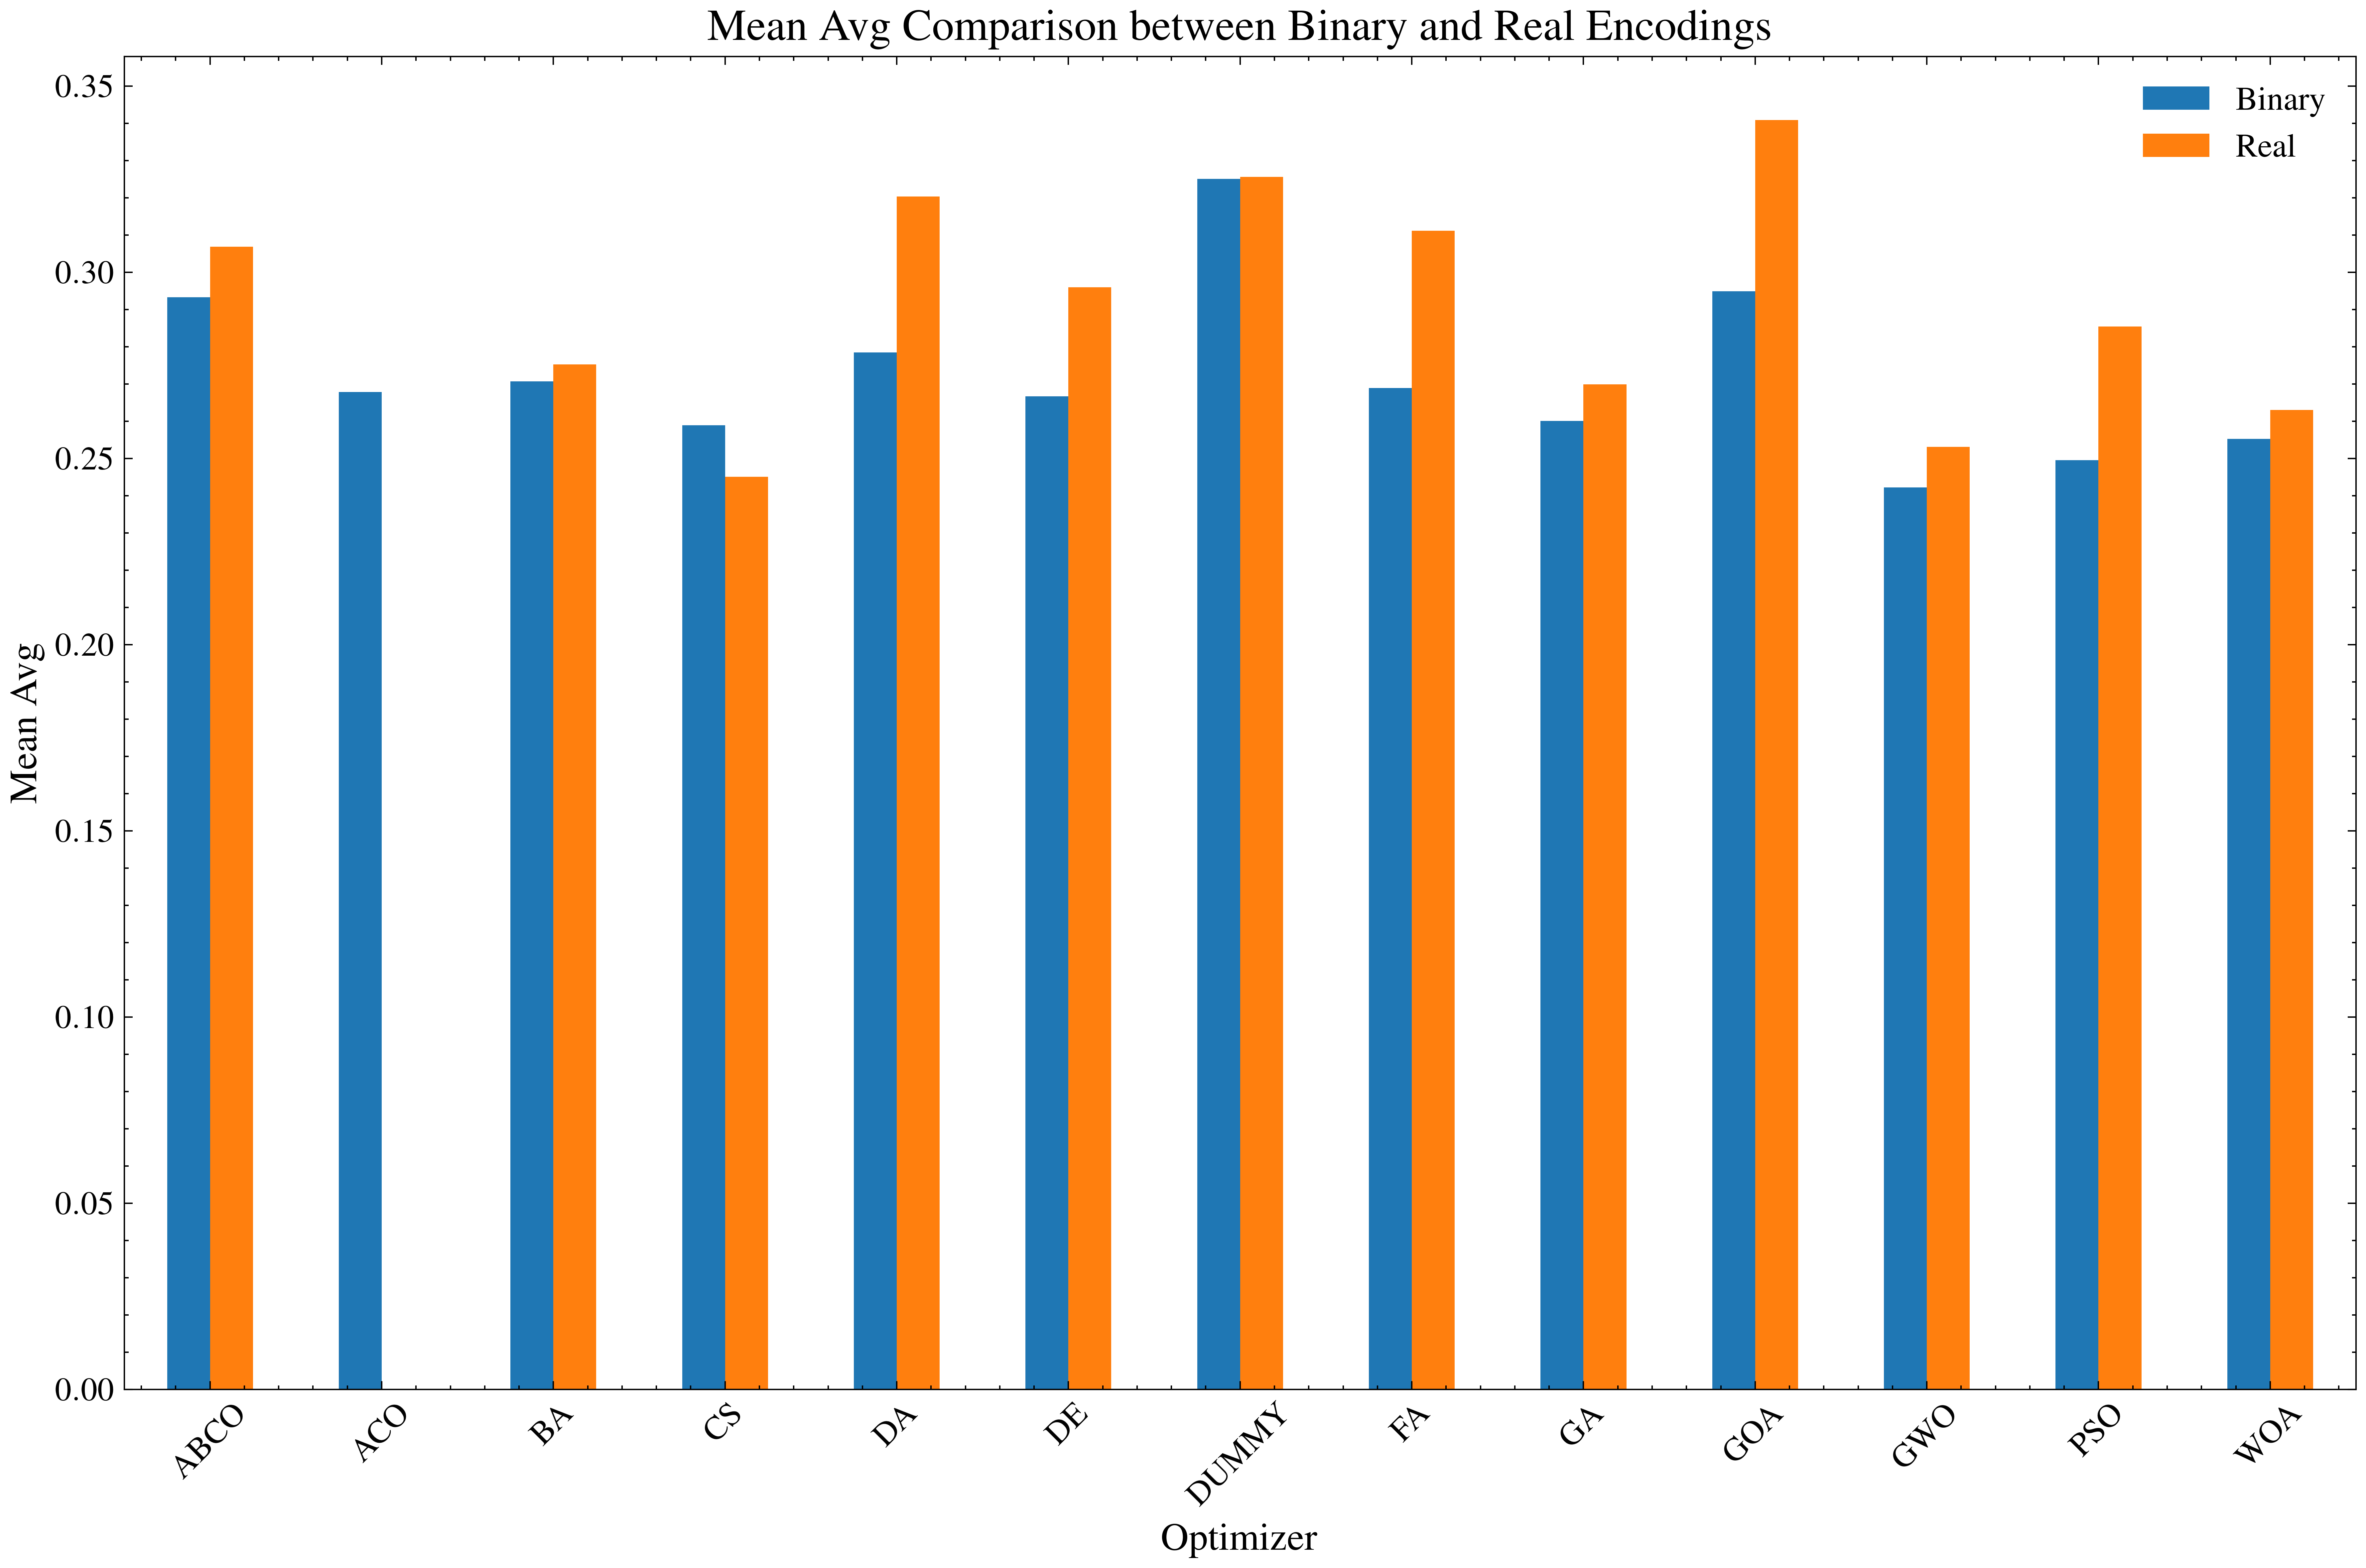
\includegraphics[width=\textwidth]{imagenes/chapter6/avg_comparison.png}
        \column{0.4\textwidth}
        \begin{itemize}
            \item<1-> Rendimiento generalmente similar
            \item<2-> Ligeras ventajas para versiones continuas en algunos casos
            \item<3-> \textcolor{blue}{Conclusión:} La mayoría de algoritmos mantienen su eficacia al ser adaptados a versiones binarias
        \end{itemize}
    \end{columns}
\end{frame}

\begin{frame}
    \frametitle{Opciones más interesantes por contexto}
    \begin{itemize}
        \item<1-> Mejor fitness general:
            \begin{itemize}
                \item Continuo: \textcolor{green}{\textbf{CS, GWO}}
                \item Binario: \textcolor{blue}{\textbf{bGWO, bPSO}}
            \end{itemize}
        \item<2-> Mejor reducción de características:
            \begin{itemize}
                \item Continuo: \textcolor{green}{\textbf{CS, GWO}} (con mucha diferencia)
                \item Binario: \textcolor{blue}{\textbf{ACO}}
            \end{itemize}
        \item<3-> Mayor eficiencia temporal:
            \begin{itemize}
                \item Continuo: \textcolor{orange}{\textbf{FA (Firefly Algorithm)}}
                \item Binario: \textcolor{orange}{\textbf{bFA (Binary Firefly Algorithm)}}
            \end{itemize}
        \item<4-> \textcolor{purple}{Conclusión:} La elección del algoritmo depende de las prioridades específicas del problema (fitness, reducción de características, eficiencia)
    \end{itemize}
\end{frame}